\documentclass{article}
\usepackage[margin=3.5cm]{geometry}
\usepackage{pdfpages}
\usepackage{graphicx}
\usepackage{zi4}
\usepackage{listings}
\usepackage{color}
\DeclareGraphicsExtensions{.pdf,.png,.jpg}	

\definecolor{mygreen}{rgb}{0,0.6,0}
\definecolor{mygray}{rgb}{0.5,0.5,0.5}
\definecolor{mymauve}{rgb}{0.58,0,0.82}

\lstdefinelanguage{UML}{
  morekeywords=[1]{
	inv, context, pre, post, and, xor, forAll, constraints, intersection, includes, size, including, not, true, false
  },
  morecomment=[l]{--}
}


\lstset{ %
  backgroundcolor=\color{white},   % choose the background color; you must add \usepackage{color} or 
  basicstyle=\footnotesize\ttfamily,
  breakatwhitespace=true,         % sets if automatic breaks should only happen at whitespace
  breaklines=true,                 % sets automatic line breaking
  captionpos=b,                    % sets the caption-position to bottom
  columns=flexible,
  commentstyle=\color{mygreen},    % comment style
  extendedchars=true,              % lets you use non-ASCII characters; for 8-bits encodings only, does not work with UTF-8
  frame=single,	                   % adds a frame around the code
  keepspaces=true,                 % keeps spaces in text, useful for keeping indentation of code (possibly needs columns=flexible)
  language=UML,                 % the language of the code
  numbers=left,                    % where to put the line-numbers; possible values are (none, left, right)
  numbersep=5pt,                   % how far the line-numbers are from the code
  numberstyle=\tiny\color{mygray}, % the style that is used for the line-numbers
  rulecolor=\color{black},         % if not set, the frame-color may be changed on line-breaks within not-black text (e.g. comments (green here))
  showstringspaces=false,          % underline spaces within strings only
  stepnumber=2,                    % the step between two line-numbers. If it's 1, each line will be numbered
  tabsize=4,	                   % sets default tabsize to 4 spaces
}

\title{Homework IV}
\author{Gregory Williams\\GW4975\\EE 382C Requirements Engineering}
\date{12/03/2015}

\begin{document}
	\maketitle
	
	\section*{4.1.1}
	The invariant is violated by \texttt{Fred} who has an \texttt{id} with length equal to \texttt{5}. The invariant \texttt{StudentIdMustBeLength4} works within the \texttt{University} context; it loads the set of all of the \texttt{students} that belong to \texttt{EnrolledAtUniversity} (i.e. are enrolled at the University) and checks each student's \texttt{id} to see if the length is equal to \texttt{4}.\\
\begin{center}
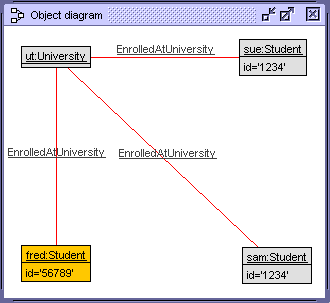
\includegraphics[width=0.5\textwidth]{Media/UniversityObjectDiagram}
\end{center}
	\section*{4.1.2}
\begin{lstlisting}
-- OCL constraints
constraints
context University
	-- A student's id number must be exactly
	-- four characters long
	inv StudentIdMustBeLength4:
		self.students->forAll( s | s.id.size() = 4 )

	-- A student's id number must be unique
	inv StudentIdMustBeUnique:
		self.students->forAll( s1, s2 | s1.id = s2.id implies s1 = s2 )
\end{lstlisting}
	
	\section*{4.1.3}
\begin{lstlisting}[language=bash]
checking invariant (2) `University::StudentIdMustBeUnique': FAILED.
-> false : Boolean
Results of subexpressions:
	University.allInstances : Set(University) = Set{@ut}
	self : University = @ut
	self.students : Set(Student) = Set{@fred,@sam,@sue}
	s1 : Student = @fred
	s1.id : String = '56789'
	s2 : Student = @fred
	s2.id : String = '56789'
	(s1.id = s2.id) : Boolean = true
	s1 : Student = @fred
	s2 : Student = @fred
	(s1 = s2) : Boolean = true
	((s1.id = s2.id) implies (s1 = s2)) : Boolean = true
	s1 : Student = @fred
	s1.id : String = '56789'
	s2 : Student = @sam
	s2.id : String = '1234'
	(s1.id = s2.id) : Boolean = false
	((s1.id = s2.id) implies (s1 = s2)) : Boolean = true
	s1 : Student = @fred
	s1.id : String = '56789'
	s2 : Student = @sue
	s2.id : String = '1234'
	(s1.id = s2.id) : Boolean = false
	((s1.id = s2.id) implies (s1 = s2)) : Boolean = true
	s1 : Student = @sam
	s1.id : String = '1234'
	s2 : Student = @fred
	s2.id : String = '56789'
	(s1.id = s2.id) : Boolean = false
	((s1.id = s2.id) implies (s1 = s2)) : Boolean = true
	s1 : Student = @sam
	s1.id : String = '1234'
	s2 : Student = @sam
	s2.id : String = '1234'
	(s1.id = s2.id) : Boolean = true
	s1 : Student = @sam
	s2 : Student = @sam
	(s1 = s2) : Boolean = true
	((s1.id = s2.id) implies (s1 = s2)) : Boolean = true
	s1 : Student = @sam
	s1.id : String = '1234'
	s2 : Student = @sue
	s2.id : String = '1234'
	(s1.id = s2.id) : Boolean = true
	s1 : Student = @sam
	s2 : Student = @sue
	(s1 = s2) : Boolean = false
	((s1.id = s2.id) implies (s1 = s2)) : Boolean = false
	self.students->forAll(s1, s2 : Student | ((s1.id = s2.id) implies (s1 = s2))) : Boolean = false
	University.allInstances->forAll(self : University | self.students->forAll(s1, s2 : Student | ((s1.id = s2.id) implies (s1 = s2)))) : Boolean = false
\end{lstlisting}
\section*{4.1.4}
\begin{lstlisting}
-- OCL constraints
constraints

context University
	-- A student may be a GraduateStudent
	-- or an UndergraduateStudent
	-- but not both
	inv StudentIsGradOrUndergradNotBoth:
		self.undergraduates->intersection(self.graduates)->isEmpty()
\end{lstlisting}
  \section*{4.1.5}
\begin{lstlisting}[language=bash]
checking invariant (1) `University::StudentIsGradOrUndergradNotBoth': FAILED.
-> false : Boolean
Results of subexpressions:
	University.allInstances : Set(University) = Set{@ut}
	self : University = @ut
	self.undergraduates : Set(Student) = Set{@sam}
	self : University = @ut
	self.graduates : Set(Student) = Set{@sam}
	self.undergraduates->intersection(self.graduates) : Set(Student) = Set{@sam}
	self.undergraduates->intersection(self.graduates)->isEmpty : Boolean = false
	University.allInstances->forAll(self : University | self.undergraduates->intersection(self.graduates)->isEmpty) : Boolean = false
\end{lstlisting}
 \section*{4.1.6}
 \begin{lstlisting}
-- OCL constraints
constraints

context University
	-- A student may not exceed the maxApprovedSemesterHours
	-- All Courses offered are assumed to have 3 credit hours
	inv StudentIsGradOrUndergradNotBoth:
		self.students->forAll(s | s.takingCourses->size() * 3 <= s.maxApprovedSemesterHours)
\end{lstlisting}
\section*{4.1.7}
\begin{lstlisting}[language=bash]
checking invariant (1) `University::StudentIsGradOrUndergradNotBoth': FAILED.
-> false : Boolean
Results of subexpressions:
	University.allInstances : Set(University) = Set{@ut}
	self : University = @ut
	self.students : Set(Student) = Set{@sam}
	s : Student = @sam
	s.takingCourses : Set(Course) = Set{@BUS311,@CS306,@E306,@EE302,@EE323,@EE338,@EE379K}
	s.takingCourses->size : Integer = 7
	3 : Integer = 3
	(s.takingCourses->size * 3) : Integer = 21
	s : Student = @sam
	s.maxApprovedSemesterHours : Integer = 18
	((s.takingCourses->size * 3) <= s.maxApprovedSemesterHours) : Boolean = false
	self.students->forAll(s : Student | ((s.takingCourses->size * 3) <= s.maxApprovedSemesterHours)) : Boolean = false
	University.allInstances->forAll(self : University | self.students->forAll(s : Student | ((s.takingCourses->size * 3) <= s.maxApprovedSemesterHours))) : Boolean = false
\end{lstlisting}
\section*{4.2.1}
\begin{lstlisting}
-- OCL constraints
constraints

context Student
	inv studentEnrolledInUniversity: self.isEnrolledAt.students->includes(self)

context Student :: drop(c : Course)
	pre studentIsRegistered: self.takingCourses->includes(c)
	pre studentHasMoreThanOneClass: self.takingCourses->size() > 1
	post studentIsNotRegistered: not self.takingCourses->includes(c)
	post studentDidNotDropOtherCoursesRegistered: self.takingCourses->including(c) = self.takingCourses@pre
	post droppedCourseNotFull: c.isFull = false
	post studentStillEnrolledInUniversity: self.isEnrolledAt = self.isEnrolledAt@pre
	post onlyThisStudentWasRemoved: c.studentsEnrolled->including(self) = c.studentsEnrolled@pre
\end{lstlisting}	
\section*{4.2.2}
\begin{lstlisting}[language=bash,otherkeywords={*,create,insert,delete,openter,opexit}]
!create ut : University
!create sam : Student
!create sue : Student
!insert (sam,ut) into EnrolledAtUniversity
!insert (sue,ut) into EnrolledAtUniversity
!create EE302 : Course
!create CS306 : Course
!create BUS311 : Course
!create EE411 : Course
!create EE379K : Course
!create E306 : Course
!create EE338 : Course
!create EE323 : Course
!insert (sam,EE302) into TakingCourse
!insert (sam,CS306) into TakingCourse
!insert (sam,BUS311) into TakingCourse
!insert (sam,EE323) into TakingCourse
!insert (sam,EE379K) into TakingCourse
!insert (sam,E306) into TakingCourse
!insert (sam,EE338) into TakingCourse
!insert (sue,EE302) into TakingCourse
!insert (sue,CS306) into TakingCourse
!insert (sue,BUS311) into TakingCourse
!insert (sue,EE323) into TakingCourse
!set EE302.isFull := true
!openter sam drop(EE302)
!delete (sam,EE302) from TakingCourse
!set EE302.isFull := false
!opexit
\end{lstlisting}
\section*{4.2.3}
\begin{lstlisting}[language=bash]
CR2.cmd> !openter sam drop(EE302)
precondition `studentIsRegistered' is true
precondition `studentHasMoreThanOneClass' is true
CR2.cmd> !delete (sam,EE302) from TakingCourse
CR2.cmd> !set EE302.isFull := false
CR2.cmd> !opexit
postcondition `studentIsNotRegistered' is true
postcondition `studentDidNotDropOtherCoursesRegistered' is true
postcondition `droppedCourseNotFull' is true
postcondition `studentEnrolledInUniversity' is true
postcondition `onlyThisStudentWasRemoved' is true
\end{lstlisting}
 \end{document}